\section{App}

\begin{figure}
\centering
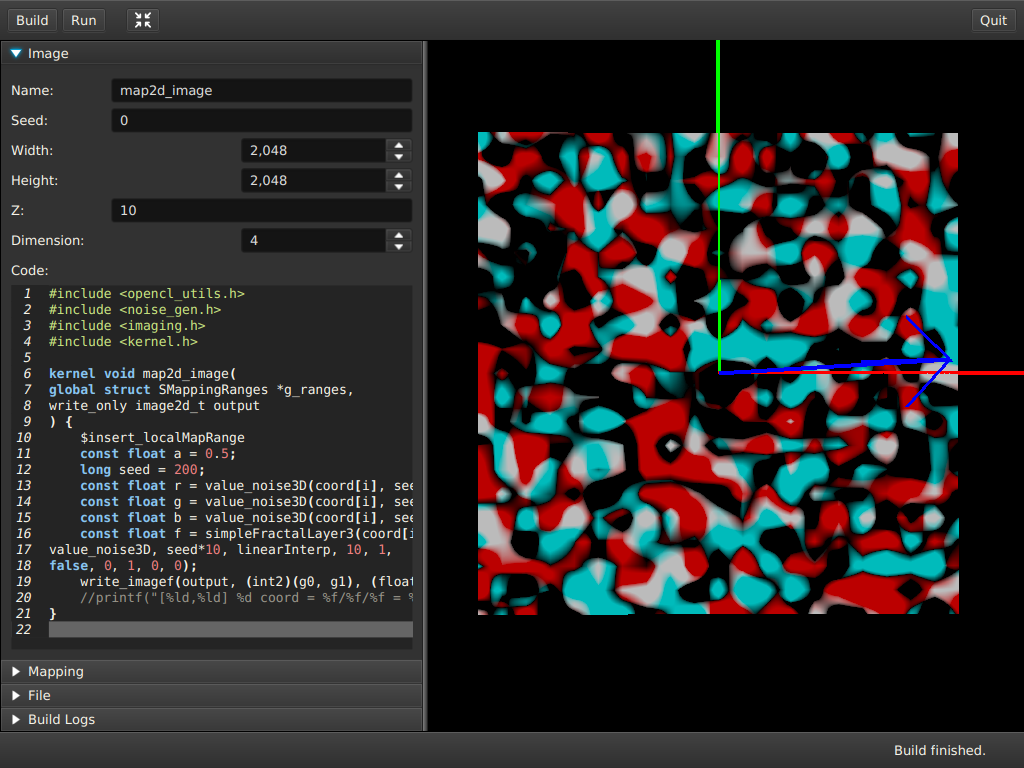
\includegraphics[width=0.4\textwidth]{Screenshot_20211121_152848.png}
\caption{Screenshot of the app version 0.0.2}\label{fig:app_screenshot}
\end{figure}

The bundled app is a graphical user interface to enter the kernel code, build
it and generate a preview of the noise image. It is implemented 
in Java and JMonkeyEngine 3. The goal of the app is to quickly prototype
noise images with kernel code. The goal is not to provide an IDE or an advanced
code editor. The app is divided into two parts. One part is to enter the kernel code and
parameters and other other part is to display the generated images.

\subsection{Toolbar}

\begin{figure}[h]
\centering
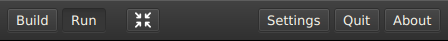
\includegraphics[width=0.4\textwidth]{imgs/toolbar-screenshot-0.png}
\caption{Toolbar}\label{fig:toolbar-screenshot-0}
\end{figure}

The toolbar have buttons for the most common functions.

\subsubsection{Build}

\begin{figure}[h]
\centering
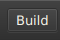
\includegraphics{imgs/toolbar-build-0.png}
\caption{Toolbar Build Button}\label{fig:toolbar-build-0}
\end{figure}

The Build button will build the kernel code and display the generated image
according to the parameters.

\subsubsection{Reset Camera}

\begin{figure}[h]
\centering

\includegraphics{imgs/toolbar-reset-camera-0.png}
\caption{Toolbar Build Button}\label{fig:toolbar-reset-camera-0}
\end{figure}

The Reset Camera button will reset the camera to the default position and zoom.
Key shortcut F10.

\subsubsection{Quit}

\begin{figure}[h]
\centering
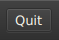
\includegraphics{imgs/toolbar-quit-0.png}
\caption{Toolbar Build Button}\label{fig:toolbar-quit-0}
\end{figure}

The Quit button will exit the app. Key shortcut Ctrl-Q.

\label{sec:image}\subsection{Image}

\begin{figure}[h]
\centering
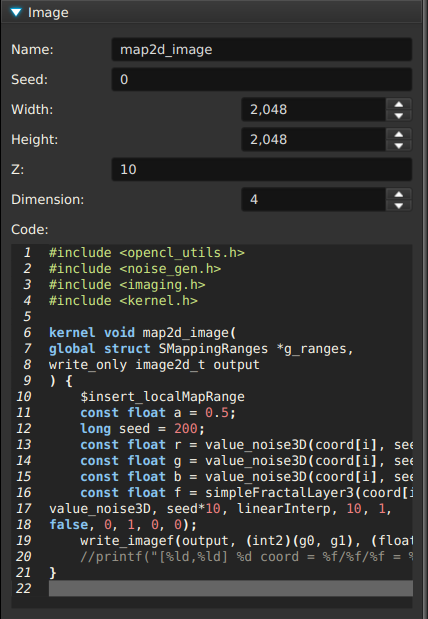
\includegraphics[width=0.4\textwidth]{imgs/main-image-0.png}
\caption{Image}\label{fig:main-image-0}
\end{figure}

The image window have the image parameters and the kernel code.

\subsubsection{Name}

The name of the kernel to build.

\subsubsection{Seed}

The seed number.

\subsubsection{Width}

The width of the image in pixels.

\subsubsection{Height}

The height of the image in pixels.

\subsubsection{Z}

The Z value.

\subsubsection{Dimension}

The count of float numbers of each coordinate. Different noise functions
expect to have the correct dimension of the coordinates available.

\begin{description}
\item[2D] requires dimension of 2 for \texttt{float2};
\item[3D] requires dimension of 4 for \texttt{float3};
\item[4D] requires dimension of 4 for \texttt{float4};
\item[6D] requires dimension of 8 for \texttt{float8};
\end{description}

\label{sec:mapping}\subsection{Mapping}

\begin{figure}[h]
\centering
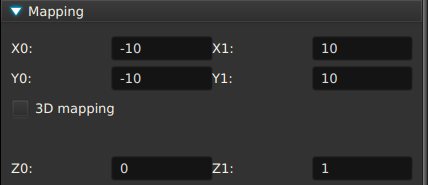
\includegraphics[width=0.4\textwidth]{imgs/main-mapping-0.png}
\caption{Image}\label{fig:main-mapping-0}
\end{figure}

The mapping window have the parameters to map coordinates.

\subsubsection{3D mapping}

If enabled then the mapping is done in 3D and the function \texttt{map3D} must be used.

\subsection{Scene Window}

\begin{figure}[h]
\centering
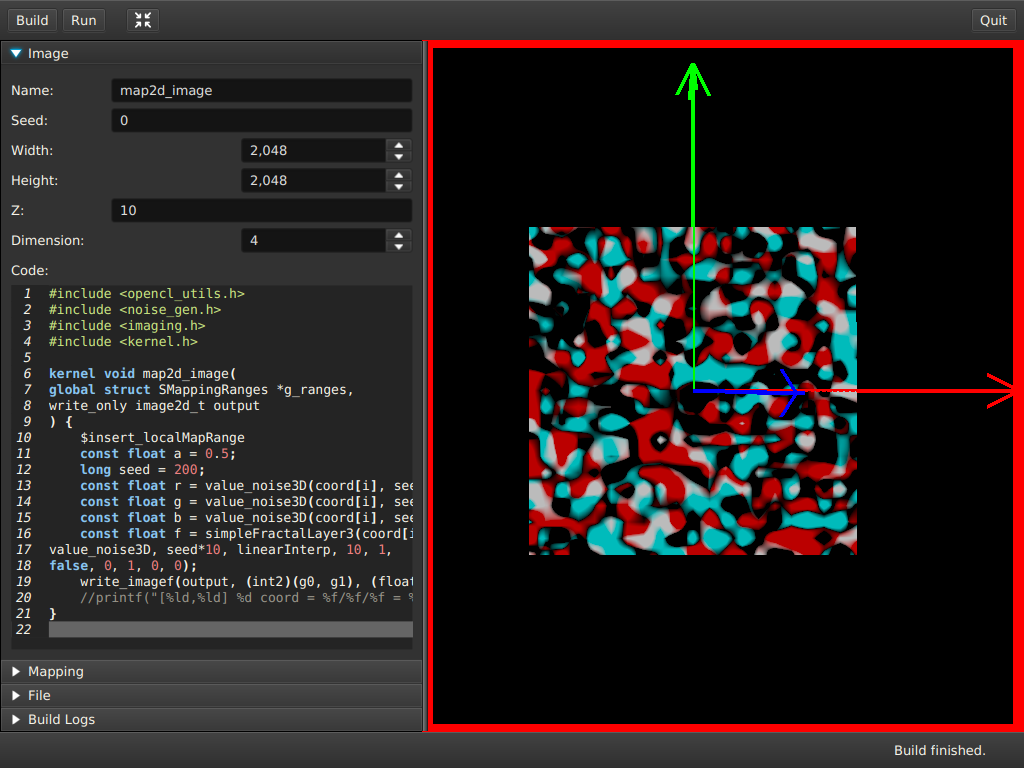
\includegraphics[width=0.4\textwidth]{imgs/main-scene-0.png}
\caption{Image}\label{fig:main-scene-0}
\end{figure}

The scene window shows the generated images. The scene can be moved and zoomed
with the mouse.

\begin{description}
\item[Middle Mouse] moving the scene;
\item[Mouse Wheel] zooming the scene;
\end{description}

